Une fonction pseudo-périodique est une fonction qui permet de décrire des phénomènes physiques du type «oscillatoire-amortis». Cette fonction peut-être le produit d'une fonction harmonique sinusoïdale et d'une fonction exponentielle décroissante, de la forme : 

\begin{equation*}
f:x\to \sin(x)\cdot \exp \left(\alpha \cdot x\right)
\end{equation*}


Le coefficient $\alpha$ doit être un réel négatif strictement pour avoir un régime amorti. On prendra dans la suite $\alpha=-0,1$. 

\bigskip{}
On souhaite obtenir le tracé ci-dessous (voir figure~\ref{PLT-001:fig:amorti}), faisant apparaître la courbe représentative de la fonction $f$ sur le segment $[0,6\pi]$, mais également les courbes enveloppes ($x\mapsto \pm \exp \left(\alpha \cdot x\right)$) et la courbe représentative de la fonction harmonique non amortie ($x\mapsto \sin x$).

\begin{figure}[h!]
\begin{center}
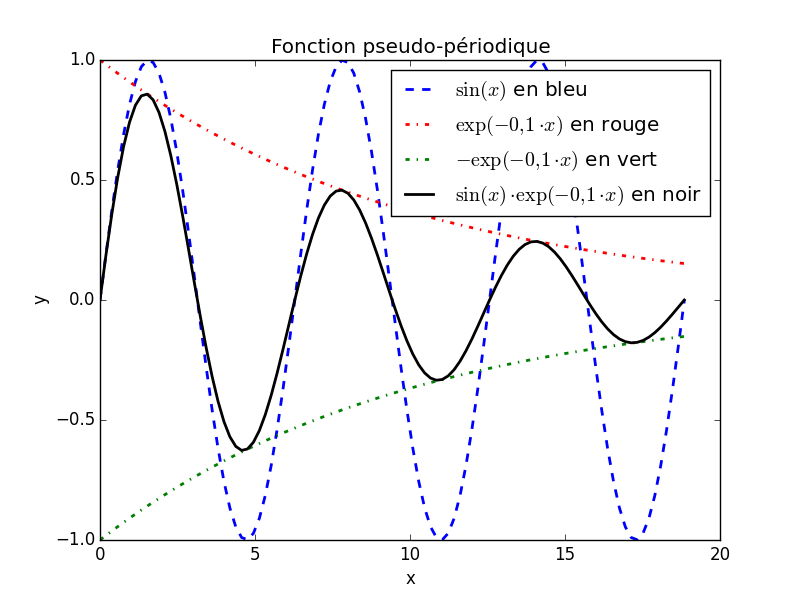
\includegraphics[width=1.0\textwidth]{pseudo_harmonique}
\caption{Tracé de $f$ et de ses enveloppes.}
\label{PLT-001:fig:amorti}
\end{center}
\end{figure}


\question{} Donner les instructions permettant de réaliser ce tracé. On veillera à bien préciser les modules utilisés et à utiliser les instructions permettant d'obtenir le tracé complet.
